\documentclass[11pt]{article}
\usepackage[margin=1.05in]{geometry}
\usepackage{amsmath,amssymb,amsthm}
\usepackage{booktabs}
\usepackage{array}
\usepackage{tabularx}
\usepackage[protrusion=true,expansion=false]{microtype}
\usepackage[table]{xcolor}
\usepackage{enumitem}
\usepackage{titlesec}
\usepackage{float}
\usepackage{tikz}
\usetikzlibrary{arrows.meta,positioning,calc,backgrounds}
\usepackage{hyperref}

\hypersetup{colorlinks=true, linkcolor=blue!60!black, urlcolor=blue!60!black, citecolor=blue!60!black}
\usepackage[skip=0.6\baselineskip, indent=0pt]{parskip}

\titleformat{\section}{\large\bfseries}{\thesection.}{0.7em}{}
\titleformat{\subsection}{\normalsize\bfseries}{\thesubsection.}{0.6em}{}

\theoremstyle{plain}
\newtheorem{proposition}{Proposition}
\theoremstyle{definition}
\newtheorem{definition}{Definition}

% ----- notation -----
\newcommand{\vmax}{V_{\max}}
\newcommand{\Tc}{T_{\mathrm{close}}}
\newcommand{\bcorr}{b_{\mathrm{corr}}}
\newcommand{\tx}[1]{\texttt{#1}}
\newcommand{\be}[2]{\langle #1\rangle_{#2}}
\newcommand{\pre}[2]{[#1]_{#2}}
\newcommand{\xo}[1]{\mathsf{x}(#1)}
\newcommand{\Ht}[1]{H_{\textsf{#1}}}
\newcommand{\Hb}[1]{H^{340}_{\textsf{#1}}}
\newcommand{\Sign}{\mathsf{Sign}}
\newcommand{\Vfy}{\mathsf{Verify}}
\newcommand{\PSign}{\mathsf{PreSign}}
\newcommand{\PVfy}{\mathsf{PreVerify}}
\newcommand{\Compl}{\mathsf{Complete}}
\newcommand{\Extr}{\mathsf{Extract}}
\newcommand{\Wots}{\mathsf{W}}
\newcommand{\kiss}{k_{\mathrm{iss}}}
\newcommand{\sid}{\mathit{sid}}
\newcommand{\owed}{\mathsf{owed}}
\newcommand{\enc}{\mathsf{enc}}
\newcommand{\PH}{P_H^{c}}
\newcommand{\Oc}{O_c}
\newcommand{\KQ}{K_{Q}^{c}}
\newcommand{\Kb}{K_{b}^{c}}
\newcommand{\Kcorr}{K_{\mathrm{corr}}^{c}}
\newcommand{\KU}{K_{U}^{c}}
\newcommand{\Acorr}{A_{\mathrm{corr}}^{c}}
\newcommand{\AU}{A_{U}^{c}}
\newcommand{\BSign}{\mathsf{BSign}}
\newcommand{\BVfy}{\mathsf{BVerify}}
\newcommand{\Enc}{\mathsf{Encrypt}}
\newcommand{\EVfy}{\mathsf{EncVerify}}
\newcommand{\Dec}{\mathsf{Decrypt}}
\newcommand{\Hg}{H_{1}}

\newcolumntype{L}{>{\raggedright\arraybackslash}X}
\renewcommand{\arraystretch}{1.3}
\makeatletter
\setlength{\@fptop}{0pt}
\setlength{\@fpsep}{1.5\baselineskip}
\setlength{\@fpbot}{0pt plus 1fil}
\makeatother

\newenvironment{algobox}[1]
  {\par\smallskip\noindent\begin{tabular}{|p{0.955\linewidth}|}\hline\textbf{#1}\\[2pt]}
  {\\\hline\end{tabular}\par\smallskip}

\title{\textbf{The grants L2}\\a Lichen L2 without global order\\[2pt]\large early draft: the countersigned exit, with BLS notes}
\author{waxwing}
\date{Version 0.4, November 2026\\[2pt]\small a companion to \emph{Lichen}, version 0.5~\cite{lichen}}

\begin{document}
\maketitle

\begin{abstract}
Lichen~\cite{lichen} enforces an L2's withdrawals through bilateral
contracts between a hub and each user, settled on Bitcoin by BABE with
the roles swapped: the user claims, and only the hub proves, if it can,
that she is owed less. This draft describes an L2 for those contracts
with no sequencer, no global ordering and no anchoring. Notes are
transparent and signed by the hub with BLS. A payment is made atomic
by a \emph{grant}: the outputs' signatures encrypted under a one-time
point $T$ that the hub opens only after the payer has signed, as in
the ecash design of~\cite{ecash} without the blinding. An exit pays
$b$, the user's claim, or $\bcorr$, the hub's correction, according to
what the user signed. The hub posts $\bcorr$ with the unlocks of the
spends it holds against her; to contest, she countersigns what it
posted, and the hub then proves $\owed \le \bcorr$ from her signatures
alone. Every value that enters the statement at exit time is under her
one-time signature, so the statement reads nothing from the chain: no
headers, no work, no inclusion proofs.

A claim names up to four notes and fallbacks, each note in 22 bytes
under one aggregate BLS signature. The deposit's note is born with the
contract, so the opening needs no swap. The open question is the
statement's cost: BLS verification in RISC Zero, unmeasured, paid by
the hub alone. This version is a proposal, not yet built; version 0.1
describes the exit as built.
\end{abstract}

\tableofcontents

\section{Setting}

A Lichen contract (\cite{lichen}, \S3) locks the hub's liquidity and the
user's deposit in one Bitcoin output, with a cap $\vmax$ and reserves
$r_A$ (hers) and $r_H$ (the hub's), and a close time $\Tc$. Amounts on
chain are counted in the contract's \emph{unit} $u$ (sats per unit): an
amount $b$ is a 4-byte word, paid out as $u\,b$ sats. It ends in one of
three ways:
\begin{itemize}[nosep]
\item \textbf{Fold}: both sign; the user is paid what she withdraws and
  her reserve.
\item \textbf{Default}: after $\Tc$, the user is paid $r_A$ and the hub
  the rest. She must withdraw or exit before.
\item \textbf{Exit}: the user posts \tx{request} with a claim of $b$
  units; she is paid $b$, or the hub's correction $\bcorr \le b$ if the
  hub proves her owed no more.
\end{itemize}

The anchored L2 (the reference L2 of~\cite{lichen}) judges a claim
against a global, anchored history. The grants L2 drops that: the hub's
book is the only ledger, and nothing is ordered beyond what each spend
names. What replaces the history is \emph{evidence the user signed}: a
claim is reduced only by spends she authorized and whose unlock she
holds.

\textbf{Contracts and credit.} A user's participation is defined by her
contract. Each contract $c$ has an L2 key $\Oc$ of its own, fresh at the
opening; the notes owned by $\Oc$ are what $c$'s exit can claim. Notes
owned by any other key (a wallet with no contract, a closed contract's
key) are the hub's IOUs with no backing on chain: credit. A wallet moves
its notes to its open contract's key with an ordinary payment to itself.

\section{Notation}\label{sec:notation}

\subsection{Group, encodings, hashes}

\begin{itemize}[nosep]
\item secp256k1: generator $G$, group order $n$. It carries Bitcoin's
  keys and the L2's owner keys.
\item BLS12-381: groups $G_1, G_2$ with generators $g_1, g_2$, order $r$,
  and the pairing $e: G_1 \times G_2 \to G_T$. $\Hg$ hashes bytes to
  $G_1$ (hash-to-curve). Points of $G_1$ are 48 bytes compressed, of
  $G_2$ 96. It carries the issuer's signatures.
\item Lower-case letters are scalars, upper-case letters points.
\item $\xo{P}$: the 32-byte x-coordinate of $P$. $\mathsf{lift}(x)$: the
  point with x-coordinate $x$ and even $y$. $P^{(33)}$: $P$ compressed.
\item Every public key is x-only (BIP340~\cite{bip340}): a key pair $(d,
  P)$ has $P = dG$ with even $y$, $d$ negated if needed.
\item $\be{v}{k}$: $v$ as $k$ bytes, big-endian. $\pre{h}{k}$: the first
  $k$ bytes of $h$. $\|$: concatenation.
\item $\Ht{tag}(p_1, \dots, p_r)$, the L2's tagged hash:
  \[
    \mathrm{SHA256}\big(\textsf{tag} \,\|\, \texttt{0x00} \,\|\, \be{|p_1|}{4}
    \,\|\, p_1 \,\|\, \cdots \,\|\, \be{|p_r|}{4} \,\|\, p_r\big),
  \]
  with tags \textsf{lichen/notes/note}, \textsf{/spend}, \textsf{/out},
  \textsf{/grant}, \textsf{/grant-commitment}, \textsf{/auth},
  \textsf{/unlock}, \textsf{/unlock-scalar}, \textsf{/issue}, written
  $\Ht{note}, \Ht{spend}, \dots$. Every part is length-prefixed, so no
  two different part lists hash alike.
\item $\Hb{tag}(x) = \mathrm{SHA256}(\mathrm{SHA256}(\textsf{tag}) \,\|\,
  \mathrm{SHA256}(\textsf{tag}) \,\|\, x)$, and BIP340's challenge $e(R,
  P, m) = \Hb{BIP0340/challenge}(\xo{R} \,\|\, \xo{P} \,\|\, m) \bmod n$,
  which depends on $R$ only through $\xo{R}$.
\end{itemize}

\subsection{Signatures}

\textbf{BIP340.} $\Sign_d(m) = (r, s)$ with $r = \xo{R}$, $R = kG$ of
even $y$, $s = k + e(R, P, m)\,d$. $\Vfy_P(m, (r, s))$ holds iff $sG =
\mathsf{lift}(r) + e(\mathsf{lift}(r), P, m)P$. 64 bytes.

\textbf{BLS}~\cite{bls} with key $k$, $K = k\,g_2$:
\begin{itemize}[nosep]
\item $\BSign_k(m) = k\,\Hg(m) \in G_1$; $\BVfy_K(m, \sigma)$ iff
  $e(\sigma, g_2) = e(\Hg(m), K)$. Unique: one signature per message.
\item \emph{Aggregate}, one signer, distinct messages: $\sigma = \sum_i
  \sigma_i$ verifies iff $e(\sigma, g_2) = e(\sum_i \Hg(m_i), K)$, two
  pairings for any number of messages. Anyone holding the $\sigma_i$
  aggregates them, without the signer.
\item \emph{Encrypted signature} under $T = t\,g_2$, made by the signer,
  who knows $t$: $\Enc_k(m, T) = (k + t)\,\Hg(m)$, a BLS signature under
  the key $K + T$. $\EVfy_K(m, T, \rho)$ iff $e(\rho, g_2) = e(\Hg(m), K
  + T)$. $\Dec(\rho, t) = \rho - t\,\Hg(m) = \BSign_k(m)$. Without $t$,
  getting $\BSign_k(m)$ from $\rho$ means computing $t\,\Hg(m)$ from
  $T$: co-CDH.
\end{itemize}

\textbf{Encryption, not adaptors.} An adaptor signature also lets
anyone \emph{extract} the secret from the pre-signature and the
signature. That is impossible for a unique signature such as
BLS~\cite{erwig}: the signer computes the signature itself, so
extraction would let it solve any instance it was handed. Here
$\rho - \BSign_k(m) = t\,\Hg(m)$, from which $t$ is a discrete log. The
design never extracts anything: $t$ always travels in the clear
(\S\ref{sec:payment}, \S\ref{sec:correct}).

\textbf{One-time signatures.} $\Wots_K(x)$ is a Winternitz signature
under the one-time key $K$ on the bytes $x$: 4-bit digits (2 a byte)
plus checksum digits, each digit given as 2 witness items (a hash
preimage and the digit itself). The chains are SHA-256 for Alice's keys, which the
statement verifies (RISC Zero accelerates SHA-256), and HASH160 for the
hub's, which only script reads. Script verifies it
digit by digit, so the digits on the stack are authenticated by the
signature, and script can compare them with other digits. A key fixed
in a leaf at the opening signs once; two different signatures under it
are an \emph{equivocation}, which some leaves punish
(\S\ref{sec:bits}).

\subsection{Keys}

\begin{center}
\begin{tabularx}{\linewidth}{llL}
\toprule
Symbol & Scope & Use \\
\midrule
$\kiss$, $I = \kiss g_2$ & the deployment (one) & the issuer's BLS key: signs every note and every grant's $T$; encrypts every grant's outputs' signatures \\
$\PH$ & contract $c$ & the hub's payment key: its half of the 2-of-2 on every link of $c$'s graph \\
$a_c$, $\Oc = a_cG$ & contract $c$ & her L2 key, fresh for $c$: owns the notes $c$'s exit claims; signs her spends of them (the \emph{owner} of $c$) \\
$P_A^c$ & contract $c$ & her half of the 2-of-2 \\
$\KQ$, $\Kb$ & contract $c$, hers & one-time: the posted claim $Q$ and $b$, in \tx{request} \\
$\Kcorr$, $\KU$ & contract $c$, the hub's & one-time: $\bcorr$ and the unlocks $U$, in \tx{correct} \\
$\Acorr$, $\AU$ & contract $c$, hers & one-time: her countersignatures on $\bcorr$ and $U$, in \tx{ack} \\
$z_S$, $t_S$, $T_S = t_S g_2$ & spend $S$ & the spend's unlock: a 16-byte seed $z_S$, its scalar $t_S$, derived by the hub \\
\bottomrule
\end{tabularx}
\end{center}

The hub derives each contract's keys from its seed and $c$, and $\kiss$
once: $I$ is common to every contract. Alice derives hers from her
wallet's key and the contract.

\section{Notes, spends and grants}

\subsection{Notes}

\begin{definition}
A \emph{note} is $N = (\mathit{id}, o, v)$: a 32-byte id, an owner (an
x-only key) and a value in sats, $v < 2^{48}$. Its short id is $\iota =
\pre{\mathit{id}}{16}$, and its digest
\[
  \delta(N) = \Ht{note}\big(\pre{\mathit{id}}{16},\ o,\ \be{v}{8}\big).
\]
$N$ is \emph{settled} when its holder has $\sigma_N = \BSign_{\kiss}(\delta(N))$,
checked by $\BVfy_I(\delta(N), \sigma_N)$.
\end{definition}

The digest names the note by its 16-byte short id, which an exit posts
(\S\ref{sec:claim}). Two notes with one short id, owner and value would
share a digest and a signature. A note's id comes from its spend's id,
which the \emph{payer} chooses, so a payer could grind two payments to
one payee to collide: at 16 bytes that is $2^{64}$ work, out of reach.
(Version 0.1 used 8 bytes, which a payer can grind in $2^{32}$, and
which made the payee's whole claim malformed. With BLS a posted note is
22 bytes, so the longer id is cheap; \S\ref{sec:claim}.)

\subsection{Spends}

\begin{definition}
A \emph{spend} $S = (N_1, \dots, N_m;\ (o'_0, v'_0), \dots, (o'_{k-1},
v'_{k-1}))$ names input notes and asks for outputs. It is well formed if
$1 \le m \le 16$, $1 \le k \le 16$, the inputs are distinct, every
$v'_j > 0$, the $o'_j$ are distinct (one output per owner), and $V =
\sum_i v_i = \sum_j v'_j$. Its id is
\[
  \sid = \Ht{spend}\big(\be{m}{4},\ \delta(N_1), \dots, \delta(N_m),\
  \be{k}{4},\ o'_0 \| \be{v'_0}{8}, \dots, o'_{k-1} \| \be{v'_{k-1}}{8}\big),
\]
and its outputs are the notes $N'_j = (\Ht{out}(\sid, \be{j}{4}),\ o'_j,\
v'_j)$, $j = 0, \dots, k-1$.
\end{definition}

The rule of one output per owner is the hub's: it refuses others.
\S\ref{sec:volume} needs it.

\subsection{Grants}\label{sec:grant}

\begin{definition}
The hub's \emph{grant} on a well-formed spend $S$ whose inputs are live
(issued, unspent) is
\[
  \Gamma = \big(\sid,\ T_S,\ \tau,\ \rho_0, \dots, \rho_{k-1}\big),
\]
where
\begin{align*}
  z_S &= \pre{\Ht{unlock}(\kiss, \sid)}{16},\qquad
  t_S = \Ht{unlock-scalar}(z_S, \be{\mathit{ctr}}{4}) \text{ for the least
  } \mathit{ctr} \text{ giving } 0 < t_S < r,\qquad T_S = t_S g_2,\\
  \tau &= \BSign_{\kiss}\big(\Ht{grant}(\sid, T_S^{(96)})\big),\\
  \rho_j &= \Enc_{\kiss}\big(\delta(N'_j), T_S\big)\quad \text{for each output } j.
\end{align*}
Its \emph{commitment}, and the message each input's owner signs, are
\[
  C = \Ht{grant-commitment}\big(\sid,\ T_S^{(96)},\ \be{k}{4},\
  \rho_0^{(48)}, \dots, \rho_{k-1}^{(48)}\big),\qquad
  \alpha = \Ht{auth}(\sid, C).
\]
The \emph{unlock} the hub hands over is the seed $z_S$; whoever holds it
computes $t_S$. A seed is 16 bytes, half a scalar, which halves what an
exit publishes (\S\ref{sec:costs}); finding $z_S$ from $T_S$ takes
$2^{128}$ work.
\end{definition}

$z_S$ is a function of the hub's key and the spend: a spend asked again
gets the same grant. $\tau$ signs $\sid$ and $T_S$ together, binding
this $T_S$ to this spend: the payer can't choose $T_S$ (and know $t_S$)
herself, and the hub can't later show another. The owners' signature
$\alpha$ stays BIP340 under their secp256k1 keys.

A grant carries nothing per contract. (Version 0.1's grants also carried
a \emph{reveal}, an adaptor pre-signature on the payer's contract's
\tx{correct}; the countersigned exit publishes unlocks directly, so it
needs none: \S\ref{sec:unlocks}.)

\subsection{A payment}\label{sec:payment}

Figure~\ref{fig:payment} shows a payment of $v$ from Alice to Bob.
Alice's wallet spends all its notes, $V$ in all: $v$ to Bob's address
$o_B$, and her change $V - v$ to her own address $o_A$ (her open
contract's key $\Oc$), left out if $v = V$. Bob need not be online.

\begin{figure}[!tbp]
\centering
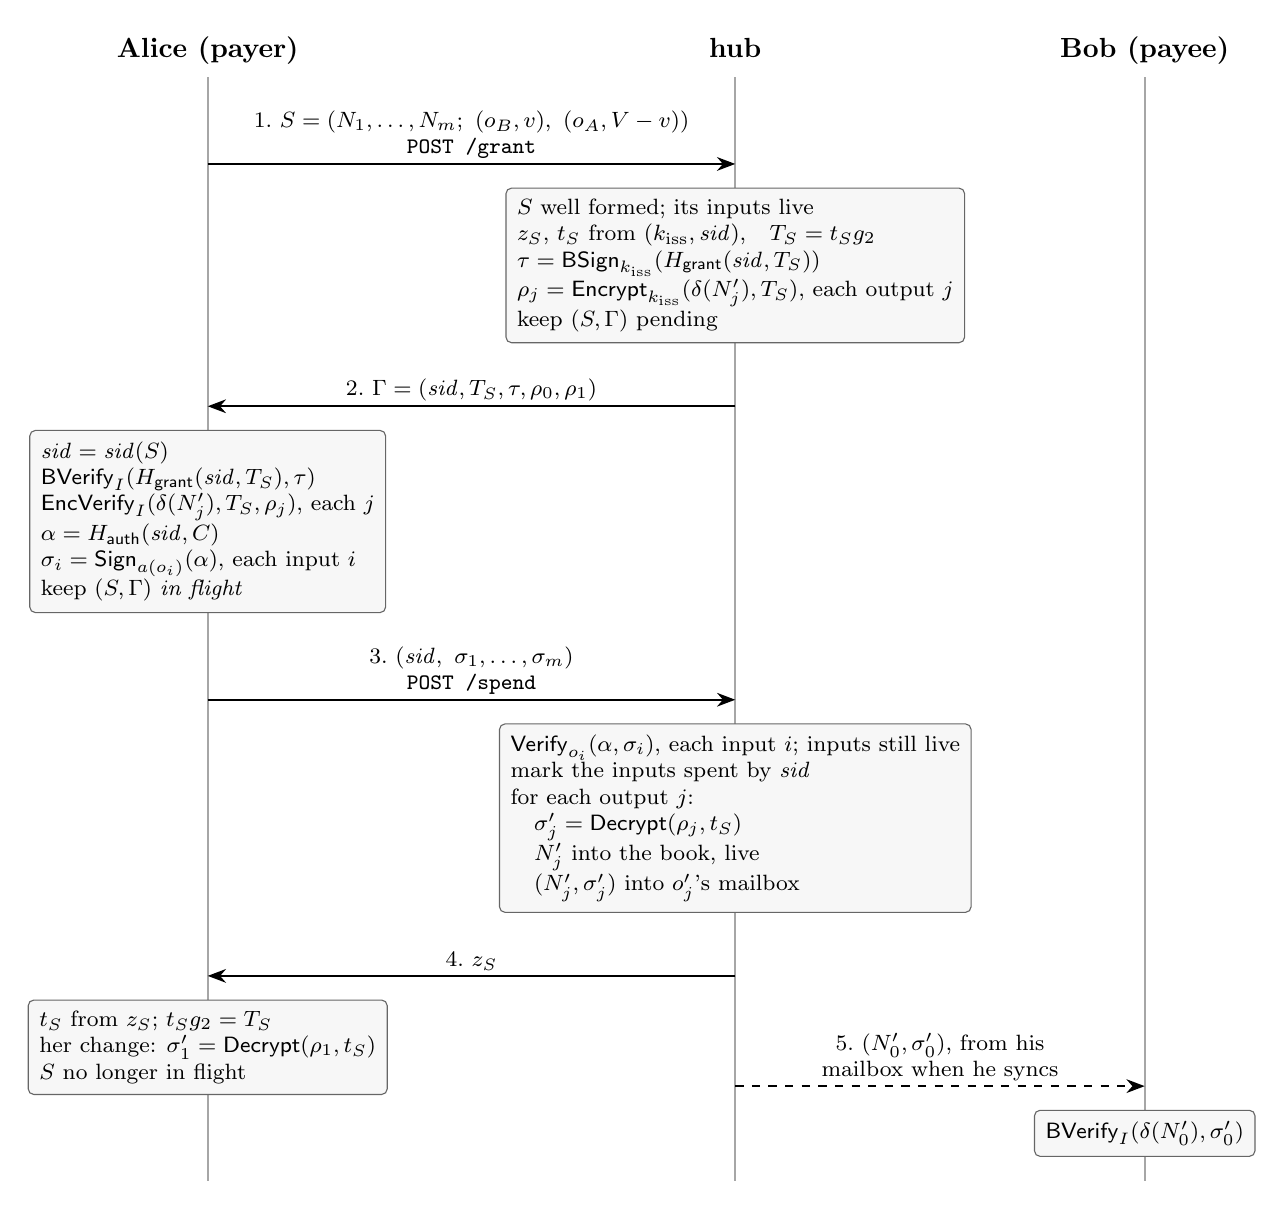
\begin{tikzpicture}[>=Stealth, font=\small,
  life/.style={draw=black!35, thick},
  box/.style={draw=black!60, fill=black!3, rounded corners=2pt, align=left, inner sep=4pt, font=\footnotesize},
  msg/.style={->, thick},
  lbl/.style={align=center, font=\footnotesize, inner sep=1.5pt}]
\coordinate (LA) at (2.6,0); \coordinate (LH) at (9.3,0); \coordinate (LB) at (14.5,0);
\node[font=\bfseries, anchor=base] at ($(LA)+(0,0.25)$) {Alice (payer)};
\node[font=\bfseries, anchor=base] at ($(LH)+(0,0.25)$) {hub};
\node[font=\bfseries, anchor=base] at ($(LB)+(0,0.25)$) {Bob (payee)};
\coordinate (y) at (0,-1.1);
\draw[msg] (LA|-y) -- node[lbl, above] {1.\ $S = (N_1, \dots, N_m;\ (o_B, v),\ (o_A, V - v))$\\ \tx{POST /grant}} (LH|-y);
\node[box, anchor=north] (b1) at ($(LH|-y)+(0,-0.3)$) {
  $S$ well formed; its inputs live\\
  $z_S$, $t_S$ from $(\kiss, \sid)$,\quad $T_S = t_S g_2$\\
  $\tau = \BSign_{\kiss}(\Ht{grant}(\sid, T_S))$\\
  $\rho_j = \Enc_{\kiss}(\delta(N'_j), T_S)$, each output $j$\\
  keep $(S, \Gamma)$ pending};
\coordinate (y) at ($(b1.south)+(0,-0.8)$);
\draw[msg] (LH|-y) -- node[lbl, above] {2.\ $\Gamma = (\sid, T_S, \tau, \rho_0, \rho_1)$} (LA|-y);
\node[box, anchor=north] (b2) at ($(LA|-y)+(0,-0.3)$) {
  $\sid = \sid(S)$\\
  $\BVfy_I(\Ht{grant}(\sid, T_S), \tau)$\\
  $\EVfy_I(\delta(N'_j), T_S, \rho_j)$, each $j$\\
  $\alpha = \Ht{auth}(\sid, C)$\\
  $\sigma_i = \Sign_{a(o_i)}(\alpha)$, each input $i$\\
  keep $(S, \Gamma)$ \emph{in flight}};
\coordinate (y) at ($(b2.south)+(0,-1.1)$);
\draw[msg] (LA|-y) -- node[lbl, above] {3.\ $(\sid,\ \sigma_1, \dots, \sigma_m)$\\ \tx{POST /spend}} (LH|-y);
\node[box, anchor=north] (b3) at ($(LH|-y)+(0,-0.3)$) {
  $\Vfy_{o_i}(\alpha, \sigma_i)$, each input $i$; inputs still live\\
  mark the inputs spent by $\sid$\\
  for each output $j$:\\
  \quad $\sigma'_j = \Dec(\rho_j, t_S)$\\
  \quad $N'_j$ into the book, live\\
  \quad $(N'_j, \sigma'_j)$ into $o'_j$'s mailbox};
\coordinate (y) at ($(b3.south)+(0,-0.8)$);
\draw[msg] (LH|-y) -- node[lbl, above] {4.\ $z_S$} (LA|-y);
\node[box, anchor=north] (b4) at ($(LA|-y)+(0,-0.3)$) {
  $t_S$ from $z_S$; $t_S g_2 = T_S$\\
  her change: $\sigma'_1 = \Dec(\rho_1, t_S)$\\
  $S$ no longer in flight};
\coordinate (y) at ($(y)+(0,-1.4)$);
\draw[msg, dashed] (LH|-y) -- node[lbl, above] {5.\ $(N'_0, \sigma'_0)$, from his\\ mailbox when he syncs} (LB|-y);
\node[box, anchor=north] (b5) at ($(LB|-y)+(0,-0.3)$) {$\BVfy_I(\delta(N'_0), \sigma'_0)$};
\coordinate (end) at ($(b5.south)+(0,-0.3)$);
\begin{scope}[on background layer]
\foreach \l in {LA,LH,LB} \draw[life] (\l) -- (\l|-end);
\end{scope}
\end{tikzpicture}
\caption{A granted payment: output 0 pays Bob $v$, output 1 returns
Alice's change. Before step 4 only the hub knows $t_S$, so the outputs'
signatures stay encrypted; after it they are ordinary settled notes.}
\label{fig:payment}
\end{figure}

\textbf{What Alice's signature covers.} $\alpha$ commits to $S$ (through
$\sid$), to $T_S$ and to every encrypted output signature, in the bytes
she checked. A cited spend in an exit is checked against exactly these
bytes (\S\ref{sec:statement}).

\textbf{Settled notes in the mailbox.} The hub delivers decrypted
signatures, not $z_S$: a settled note checks under $I$ alone; $z_S$
would also need the grant, which shows Alice's change and key to Bob;
and the mailbox's other deliveries (notes issued outright, a
withdrawal's change) are settled notes too. Alice, who holds the grant,
gets $z_S$ itself.

\textbf{In flight.} From step 3 until she has $z_S$, Alice keeps $(S,
\Gamma)$ and her inputs. The hub may say it never recorded $S$; she
can't tell. She keeps claiming her inputs, with $S$ as a
\emph{fallback} (\S\ref{sec:claim}): if the hub uses $S$ against that
claim, it must hand her $z_S$, and her change counts instead.

\textbf{What atomicity means here.} Once Alice signs, the hub may record
$S$ or not.
\begin{itemize}[nosep]
\item Not recorded: the hub alone knows $t_S$, so the outputs never
  settle, and her inputs stay hers.
\item Recorded, $z_S$ given (to her, or the settled note to Bob): both
  sides are paid.
\item Recorded, $z_S$ withheld from both: the hub holds her inputs and
  pays no one; Bob has nothing to deliver goods against. Her exit
  settles it: the hub can count $S$ against her claim only by publishing
  $z_S$ in \tx{correct}; she then decrypts $\sigma'_0$ and hands Bob
  his note. Otherwise $S$ doesn't count, and her claim is owed its
  inputs.
\end{itemize}
Bob is paid when he holds $\sigma'_0$, and Alice can always produce it
once she has $z_S$.

\subsection{The wallet's policy}

A payment spends all the wallet's notes, to the payee and one change
note back. The wallet merges (a payment to itself, at its address) once
it holds more than 2 notes, or any note under a key other than its
address. Its address is its open contract's key $\Oc$, or its base key
if it has none. It refuses to pay itself any other way.

\textbf{Receiving offline.} Payments accumulate in the mailbox while
Bob is away, each one settled. Only those his exit can claim are
protected: at most 4 notes (\S\ref{sec:claim}), his largest, until he
merges. A merge is a spend, so it needs the hub; a hub that turns
hostile while he holds more leaves the rest as credit.

\section{The contract}

\subsection{Opening}\label{sec:opening}

The opening follows~\cite{lichen} (Figure~\ref{fig:opening}). Her
deposit becomes an L2 balance through the \emph{mint}, a note the
contract itself vouches for:
\begin{enumerate}[nosep]
\item Alice derives a fresh key $a_c$, $\Oc = a_cG$, and pays her
  deposit $v_D$ to a coin $O_D$: a 2-of-2 of hers and the hub's, or her
  refund alone after a timeout.
\item She asks for a contract with owner $\Oc$. The hub refuses an $\Oc$
  it has seen before: the owner of a contract, or of any note, pending
  or issued.
\item The setup (\cite{lichen}): the statement fixed by its journal $J$
  (\S\ref{sec:journal}), which binds her one-time keys and the mint's
  value $v_0$, her deposit less the opening's fee; the BABE instances
  garbled by Alice and kept by the hub by cut-and-choose.
\item The hub's offer: the funding $F$, spending $O_D$ and the hub's
  coins into the contract output, and its pre-signatures on the graph.
\item Alice signs the graph and $F$'s spend of $O_D$.
\item The hub adds its signature and broadcasts $F$.
\end{enumerate}
\textbf{The mint} is the note
\[
  N_0 = \big(\Ht{issue}(\texttt{"mint"} \,\|\, \be{c}{4}),\ \Oc,\ v_0\big).
\]
It has no signature: its evidence is the contract, whose journal binds
$v_0$, and a claim includes it by a flag (\S\ref{sec:claim}). The hub
enters it in its book once $F$ confirms, and her spends of it are
granted like any other. So the swap is atomic by the contract's
existence: if $F$ confirms, the contract exists and $N_0$ with it; if
it never confirms, there is neither, and Alice refunds $O_D$ after its
timeout. Nothing needs to be extracted, and a lost answer from the hub
costs her nothing: $F$ on chain is enough. The hub must not record a
spend of $N_0$ before $F$ confirms, which is its own risk.

\begin{figure}[!tbp]
\centering
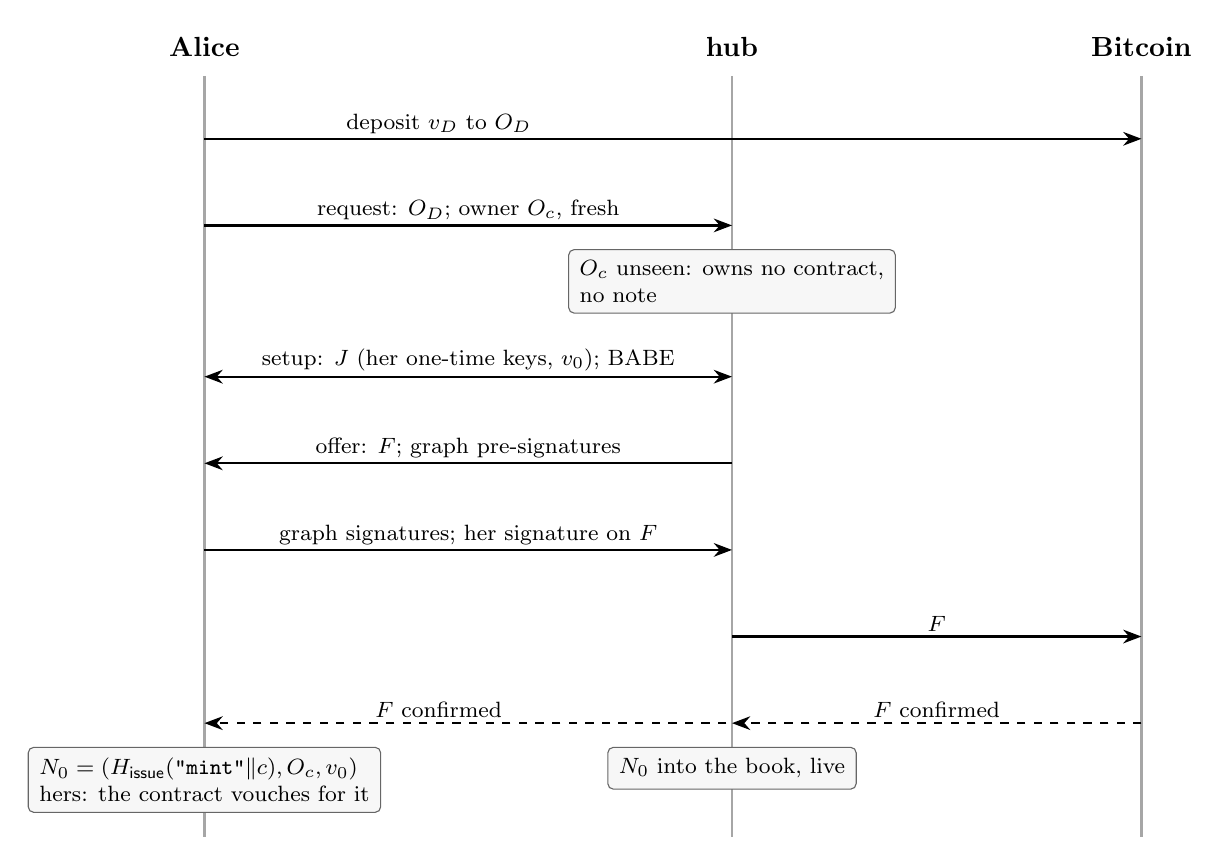
\begin{tikzpicture}[>=Stealth, font=\small,
  life/.style={draw=black!35, thick},
  box/.style={draw=black!60, fill=black!3, rounded corners=2pt, align=left, inner sep=4pt, font=\footnotesize},
  msg/.style={->, thick},
  lbl/.style={align=center, font=\footnotesize, inner sep=1.5pt}]
\coordinate (LA) at (2.6,0); \coordinate (LH) at (9.3,0); \coordinate (LB) at (14.5,0);
\node[font=\bfseries, anchor=base] at ($(LA)+(0,0.25)$) {Alice};
\node[font=\bfseries, anchor=base] at ($(LH)+(0,0.25)$) {hub};
\node[font=\bfseries, anchor=base] at ($(LB)+(0,0.25)$) {Bitcoin};
\coordinate (y) at (0,-0.8);
\draw[msg] (LA|-y) -- node[lbl, above, pos=0.25] {deposit $v_D$ to $O_D$} (LB|-y);
\coordinate (y) at ($(y)+(0,-1.1)$);
\draw[msg] (LA|-y) -- node[lbl, above] {request: $O_D$; owner $\Oc$, fresh} (LH|-y);
\node[box, anchor=north] (b1) at ($(LH|-y)+(0,-0.3)$) {$\Oc$ unseen: owns no contract,\\ no note};
\coordinate (y) at ($(b1.south)+(0,-0.8)$);
\draw[msg, <->] (LA|-y) -- node[lbl, above] {setup: $J$ (her one-time keys, $v_0$); BABE} (LH|-y);
\coordinate (y) at ($(y)+(0,-1.1)$);
\draw[msg] (LH|-y) -- node[lbl, above] {offer: $F$; graph pre-signatures} (LA|-y);
\coordinate (y) at ($(y)+(0,-1.1)$);
\draw[msg] (LA|-y) -- node[lbl, above] {graph signatures; her signature on $F$} (LH|-y);
\coordinate (y) at ($(y)+(0,-1.1)$);
\draw[msg] (LH|-y) -- node[lbl, above] {$F$} (LB|-y);
\coordinate (y) at ($(y)+(0,-1.1)$);
\draw[msg, dashed] (LB|-y) -- node[lbl, above] {$F$ confirmed} (LH|-y);
\node[box, anchor=north] (b3) at ($(LH|-y)+(0,-0.3)$) {$N_0$ into the book, live};
\draw[msg, dashed] (LB|-y) -- node[lbl, above, pos=0.75] {$F$ confirmed} (LA|-y);
\node[box, anchor=north] (b4) at ($(LA|-y)+(0,-0.3)$) {$N_0 = (\Ht{issue}(\texttt{"mint"} \| c), \Oc, v_0)$\\ hers: the contract vouches for it};
\coordinate (end) at ($(b4.south)+(0,-0.3)$);
\begin{scope}[on background layer]
\foreach \l in {LA,LH,LB} \draw[life] (\l) -- (\l|-end);
\end{scope}
\end{tikzpicture}
\caption{The opening: the mint $N_0$ exists exactly when the contract
does, so the deposit and the L2 balance need no swap.}
\label{fig:opening}
\end{figure}

\subsection{The journal}\label{sec:journal}

The statement's only public input, fixed at the opening, is
\begin{align*}
  J &= \be{c}{4} \,\|\, D,\\
  D &= \mathrm{SHA256}\big(\texttt{"lichen/grants/contract"} \,\|\,
  I^{(96)} \,\|\, \xo{\Oc} \,\|\, \be{u}{8} \,\|\, \be{v_0}{8} \,\|\, \kappa\big),\\
  \kappa &= \mathrm{SHA256}\big(\KQ \,\|\, \Kb \,\|\, \Acorr \,\|\, \AU\big),
\end{align*}
$\kappa$ hashing Alice's four one-time public keys (each the list of its
chains' ends). $D$ binds the issuer, the owner, the unit, the mint's
value, and the keys under which every exit-time value reaches the
statement (\S\ref{sec:statement}). Without the owner, a hub could prove
against another key and call every claim malformed; without the unit,
it could prove at another $u$.

\subsection{The dispute graph}\label{sec:graph}

Every transaction has one input; every link has one output that carries
the value on, plus an anchor for fees. Each link is signed by the 2-of-2
$(P_A^c, \PH)$, pre-signed at the opening; each output has its
terminals. $\epsilon$ is a short relative lock on every link, so that a
link can't confirm in its parent's block. Figure~\ref{fig:graph} shows
the graph.

\begin{figure}[!tbp]
\centering
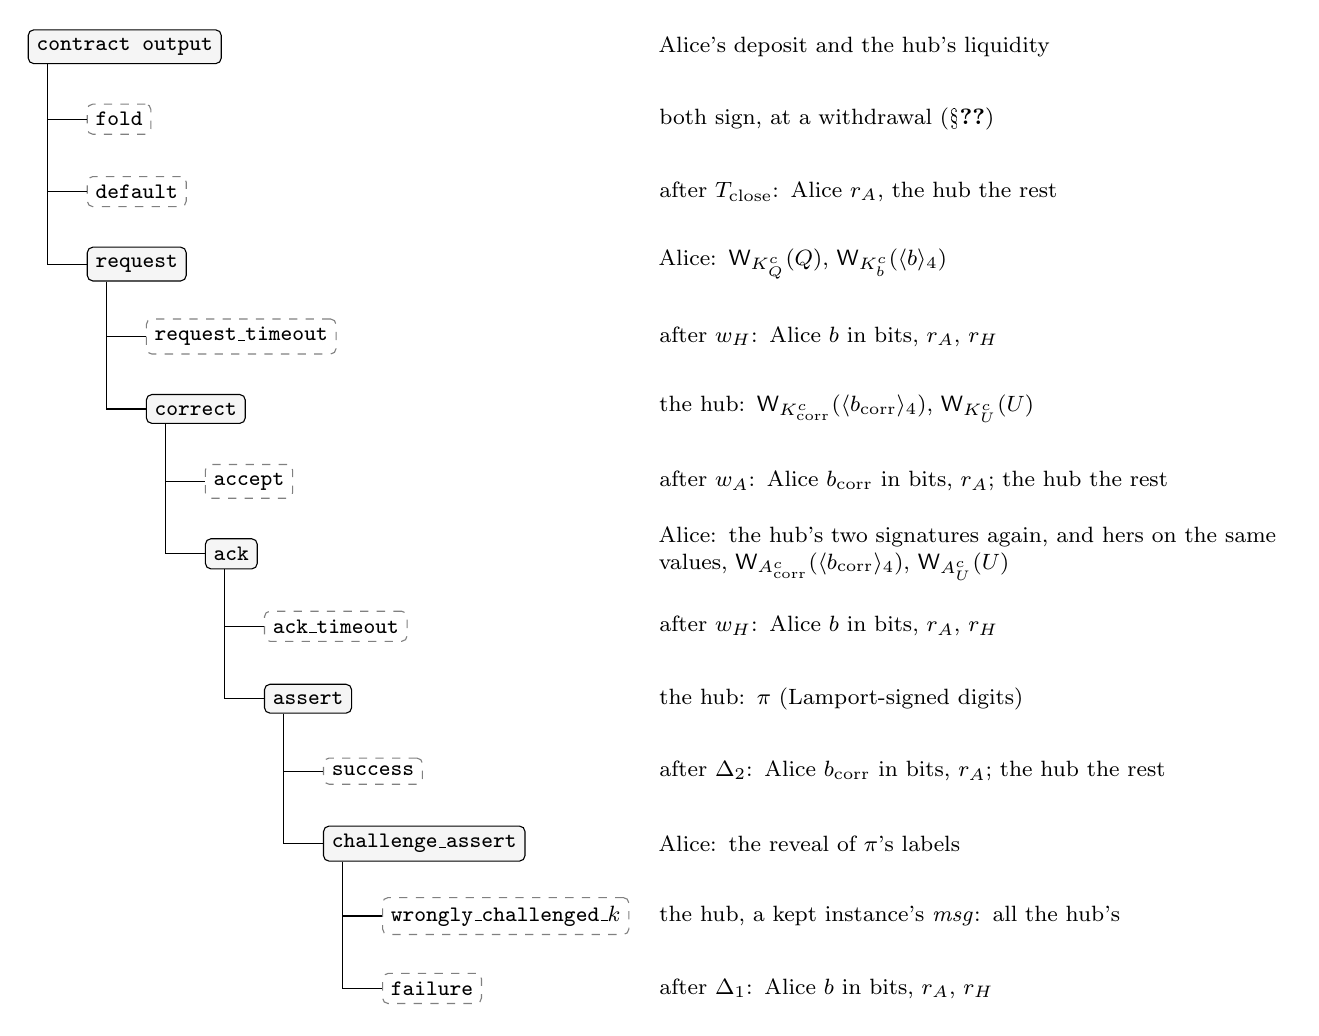
\begin{tikzpicture}[font=\footnotesize,
  link/.style={draw, rounded corners=2pt, inner sep=3pt, fill=black!4, font=\footnotesize\ttfamily, anchor=west},
  term/.style={draw=black!50, dashed, rounded corners=2pt, inner sep=3pt, font=\footnotesize\ttfamily, anchor=west},
  ann/.style={anchor=west, align=left, text width=7.9cm, font=\footnotesize}]
\def\dx{0.75}\def\dy{0.92}\def\ax{7.9}
\node[link] (c)  at (0*\dx, 0)       {contract output};
\node[term] (fo) at (1*\dx, -1*\dy)  {fold};
\node[term] (de) at (1*\dx, -2*\dy)  {default};
\node[link] (rq) at (1*\dx, -3*\dy)  {request};
\node[term] (rt) at (2*\dx, -4*\dy)  {request\_timeout};
\node[link] (co) at (2*\dx, -5*\dy)  {correct};
\node[term] (ac) at (3*\dx, -6*\dy)  {accept};
\node[link] (ak) at (3*\dx, -7*\dy)  {ack};
\node[term] (at) at (4*\dx, -8*\dy)  {ack\_timeout};
\node[link] (as) at (4*\dx, -9*\dy)  {assert};
\node[term] (su) at (5*\dx, -10*\dy) {success};
\node[link] (ch) at (5*\dx, -11*\dy) {challenge\_assert};
\node[term] (wc) at (6*\dx, -12*\dy) {wrongly\_challenged\_$k$};
\node[term] (fa) at (6*\dx, -13*\dy) {failure};
\foreach \p/\q in {c/fo,c/de,c/rq,rq/rt,rq/co,co/ac,co/ak,ak/at,ak/as,as/su,as/ch,ch/wc,ch/fa}
  \draw ($(\p.south west)+(0.25,0)$) |- (\q.west);
\node[ann] at (\ax, 0)         {Alice's deposit and the hub's liquidity};
\node[ann] at (\ax, -1*\dy)    {both sign, at a withdrawal (\S\ref{sec:withdrawal})};
\node[ann] at (\ax, -2*\dy)    {after $\Tc$: Alice $r_A$, the hub the rest};
\node[ann] at (\ax, -3*\dy)    {Alice: $\Wots_{\KQ}(Q)$, $\Wots_{\Kb}(\be{b}{4})$};
\node[ann] at (\ax, -4*\dy)    {after $w_H$: Alice $b$ in bits, $r_A$, $r_H$};
\node[ann] at (\ax, -5*\dy)    {the hub: $\Wots_{\Kcorr}(\be{\bcorr}{4})$, $\Wots_{\KU}(U)$};
\node[ann] at (\ax, -6*\dy)    {after $w_A$: Alice $\bcorr$ in bits, $r_A$; the hub the rest};
\node[ann] at (\ax, -7*\dy)    {Alice: the hub's two signatures again, and hers on the same values, $\Wots_{\Acorr}(\be{\bcorr}{4})$, $\Wots_{\AU}(U)$};
\node[ann] at (\ax, -8*\dy)    {after $w_H$: Alice $b$ in bits, $r_A$, $r_H$};
\node[ann] at (\ax, -9*\dy)    {the hub: $\pi$ (Lamport-signed digits)};
\node[ann] at (\ax, -10*\dy)   {after $\Delta_2$: Alice $\bcorr$ in bits, $r_A$; the hub the rest};
\node[ann] at (\ax, -11*\dy)   {Alice: the reveal of $\pi$'s labels};
\node[ann] at (\ax, -12*\dy)   {the hub, a kept instance's \textit{msg}: all the hub's};
\node[ann] at (\ax, -13*\dy)   {after $\Delta_1$: Alice $b$ in bits, $r_A$, $r_H$};
\end{tikzpicture}

\bigskip
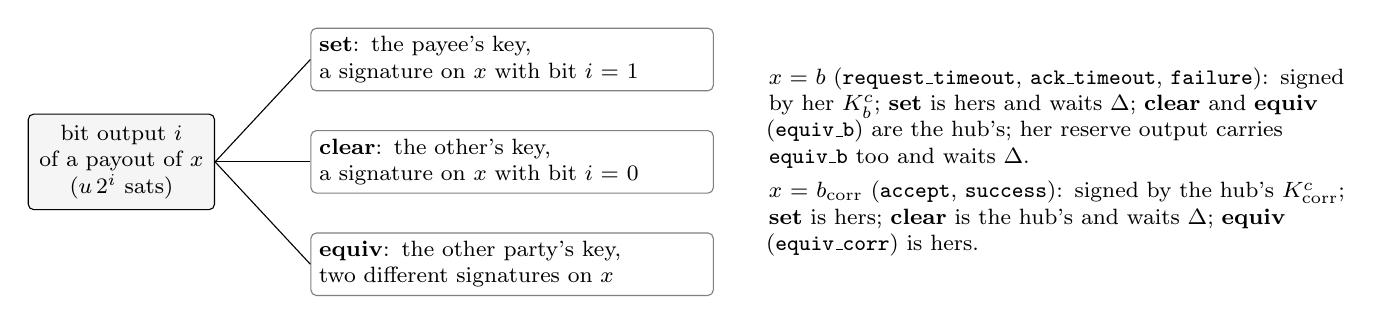
\begin{tikzpicture}[font=\footnotesize,
  bout/.style={draw, rounded corners=2pt, inner sep=4pt, fill=black!4, align=center},
  leaf/.style={draw=black!50, rounded corners=2pt, inner sep=3pt, align=left, text width=4.9cm}]
\node[bout] (o) at (0,0) {bit output $i$\\ of a payout of $x$\\ ($u\,2^i$ sats)};
\node[leaf, anchor=west] (l1) at (2.4, 1.3)  {\textbf{set}: the payee's key,\\ a signature on $x$ with bit $i$ = 1};
\node[leaf, anchor=west] (l2) at (2.4, 0)    {\textbf{clear}: the other's key,\\ a signature on $x$ with bit $i$ = 0};
\node[leaf, anchor=west] (l3) at (2.4, -1.3) {\textbf{equiv}: the other party's key,\\ two different signatures on $x$};
\draw (o.east) -- (l1.west); \draw (o.east) -- (l2.west); \draw (o.east) -- (l3.west);
\node[anchor=west, align=left, text width=7.4cm] at (8.1, 0) {
  $x = b$ (\tx{request\_timeout}, \tx{ack\_timeout}, \tx{failure}): signed by her $\Kb$; \textbf{set} is hers and waits $\Delta$; \textbf{clear} and \textbf{equiv} (\tx{equiv\_b}) are the hub's; her reserve output carries \tx{equiv\_b} too and waits $\Delta$.\\[3pt]
  $x = \bcorr$ (\tx{accept}, \tx{success}): signed by the hub's $\Kcorr$; \textbf{set} is hers; \textbf{clear} is the hub's and waits $\Delta$; \textbf{equiv} (\tx{equiv\_corr}) is hers.};
\end{tikzpicture}
\caption{Above, a contract's graph: solid boxes carry the value on,
dashed ones are terminals; each edge is a pre-signed spend of its
parent's output, with its poster and witness, or its relative
timelock. Below, one bit output of a payout: the signer of $x$ waits
$\Delta$, so the other party can show an equivocation first.}
\label{fig:graph}
\end{figure}

\subsection{Bits and equivocation}\label{sec:bits}

A payout of $x$ units (in \tx{request\_timeout}, \tx{accept},
\tx{ack\_timeout}, \tx{success} or \tx{failure}) has, for each bit
position $i$ of the contract, an output of $u\,2^i$ sats. Each is spent
by presenting the one-time signature on $x$ \emph{again}, its leaf
reading bit $i$ from the digits: the payee takes it if the bit is set,
the other party if clear. Whoever signed $x$ could present a signature
on another value, so the other party has a third leaf, taking the
output on two different signatures under that key, and the signer's own
leaf waits $\Delta$ to give it time (Figure~\ref{fig:graph}, below).

This is also why $b$ has its own key, apart from the claim's: each bit
output re-presents $\Wots_{\Kb}(\be{b}{4})$, about 20 witness items; with
$b$ inside the claim's signature, every bit output would verify some
800.

The one-time keys that sign values the bit outputs don't read ($\KQ$,
$\KU$, $\Acorr$, $\AU$) need no equivocation leaf: a second signature
under one of them has nowhere on chain to do harm. (Off chain it can:
\S\ref{sec:who}.)

\textbf{Windows} on Mutinynet (30\,s blocks): $w_H$ for the hub's moves
(\tx{correct} after \tx{request}; \tx{assert} after \tx{ack}, which must
cover proving: \S\ref{sec:costs}); $w_A$ for her \tx{ack} (2,880 blocks,
a day, as her challenge); $\Delta_2$ = 2,880 for her challenge;
$\Delta_1$ = 240 for the hub's answer.

\textbf{No penalty.} \tx{accept} and \tx{success} return her reserve
whatever $\bcorr$. A false claim
gains her nothing (she is paid what she is owed) and costs the hub one
dispute; a penalty would also strike an honest wallet restored from a
stale backup.

\subsection{Withdrawal}\label{sec:withdrawal}

Alice hands the hub a full claim (\S\ref{sec:claim}) signed with $a_c$.
The hub takes it if its book owes it in full: it marks the notes as
taken by this contract's claim, issues their value beyond $u\,b$ back to
$\Oc$ as change (now credit), and both sign the fold. If the hub takes
the claim and won't fold, her exit posts the same claim; a claim on the
same contract never counts against itself.

\section{The exit}\label{sec:exit}

\subsection{The claim}\label{sec:claim}

\begin{definition}
A \emph{claim} on contract $c$ is $(b;\ \mu;\ N_1, \dots, N_n;\ \sid_1,
\dots, \sid_f)$: a flag $\mu \in \{0, 1\}$, whether it includes the mint
$N_0$; settled notes of $\Oc$ other than the mint, with distinct short
ids, each with $\sigma_{N_i}$; $f$ \emph{fallbacks}, the ids of her
spends in flight that take any of its notes, with distinct
$\pre{\sid_l}{8}$; with $\mu + n \ge 1$, $\mu + n + f \le 4$, and $b \le
\lfloor (\mu v_0 + \sum_i v_i) / u\rfloor$.
\end{definition}

$\mu + n + f \le 4$ is the exit's capacity: at most 4 spends ever need
citing (\S\ref{sec:volume}), and \tx{correct} publishes 4 unlock seeds.
The wallet picks the largest of $\Oc$'s notes that fit with the
fallbacks they need, and sets $b$ to what she withdraws.

\textbf{The posted claim} $Q$ is what \tx{request} carries, exactly
$L_Q = 137$ bytes:
\[
  Q = \be{64\mu + 8n + f}{1} \,\big\|\, \mathop{\big\|}_{i=1}^{n}
  \big(\pre{\mathit{id}_i}{16} \,\|\, \be{v_i}{6}\big)
  \,\big\|\, \sigma^{(48)} \,\big\|\, \mathop{\big\|}_{l=1}^{f} \pre{\sid_l}{8}
  \,\big\|\, 0^{\ast}:
\]
the flag and counts; per note its short id and value, 22 bytes; the
aggregate $\sigma$ of the hub's signatures on them (the identity if $n
= 0$); each fallback's first 8 bytes; zeros to $L_Q$. Four signed notes
take $1 + 4 \cdot 22 + 48 = 137$ bytes, the most. The mint, the
contract ($c$, $\Oc$, $u$) and $v_0$ are not in $Q$: the statement
takes them from the journal. $b$ is not in $Q$: \tx{request} signs it
under its own key (\S\ref{sec:bits}).

\textbf{Aggregation.} With $m_i = \delta(N_i) =
\Ht{note}(\pre{\mathit{id}_i}{16}, \Oc, \be{v_i}{8})$, Alice sets $\sigma
= \sum_i \sigma_{N_i}$, and the claim's signature holds iff
\[
  e(\sigma, g_2) = e\Big(\sum_{i=1}^{n} \Hg(m_i),\ I\Big).
\]
One signer and distinct messages (the short ids are distinct) make this
sound: with $\Hg$ a random oracle, signatures Alice holds can't be
recombined into an aggregate over a note she wasn't issued. The
aggregate says only that all are valid, which is all the statement
asks.

\textbf{Fallbacks' 8 bytes.} A fallback is only matched against spends
the hub cites, each one she signed, and each prefix revives once
whatever spends share it (Algorithm~1). So a prefix collision adds no
candidates, and whatever it revives is change of a spend of hers that
the hub chose to cite: hers, unless a later cited spend kills it.

\textbf{\tx{request}'s witness}: $\Wots_{\KQ}(Q)$ and
$\Wots_{\Kb}(\be{b}{4})$, under the 2-of-2's two signatures: $2(2 \cdot
137 + 4) + 2(8 + 2) + 2 = 578$ stack items, well inside Bitcoin's
1,000.

\subsection{The hub's correction}\label{sec:correct}

When \tx{request} appears, the hub:
\begin{enumerate}[nosep]
\item reads $b$ and $Q$ from \tx{request}'s witness, and maps each posted
  note $(\iota_i, v_i)$, and the mint if flagged, to its book (owner
  $\Oc$), and each fallback
  $\pre{\sid_l}{8}$ to a recorded spend;
\item gathers the evidence: for each claimed note the recorded spend that
  took it, and through a spend the claim names a fallback, that spend's
  output to $\Oc$ in turn;
\item computes $x = \owed(\cdot)$ (Algorithm~1) with the statement's own
  function, taking as $U$ the unlocks of the spends it cites;
\item takes the claim into its book at $x$, in the same step: its live
  notes (and revived change) are marked taken, so no later spend of them
  is recorded;
\item if $x = b$: does nothing, and \tx{request\_timeout} pays $b$;
\item otherwise posts \tx{correct} with $\bcorr = x$ and
  \[
    U = z_{S_1} \,\|\, \cdots \,\|\, z_{S_q} \,\|\, 0^{16(4 - q)},
  \]
  the unlock seeds of the $q \le 4$ spends it cites, 64 bytes, each
  under its one-time key: $\Wots_{\Kcorr}(\be{\bcorr}{4})$ and
  $\Wots_{\KU}(U)$.
\end{enumerate}

\subsection{Alice's answer: accept or countersign}\label{sec:ack}

\tx{correct} is public, and so is $U$: Alice reads every seed in it.
For each spend $(S, \Gamma)$ she has in flight, she looks for $z \in U$
whose scalar $t$ has $t\,g_2 = T_S$; for each found, she decrypts every
$\rho_j$, hands Bob his note, and drops $S$ from in flight. Then:
\begin{itemize}[nosep]
\item \textbf{Accept}: she does nothing. After $w_A$, \tx{accept} pays
  her $\bcorr$ and $r_A$. No proof.
\item \textbf{Contest}: she posts \tx{ack}, whose leaf verifies
  \[
    \Wots_{\Kcorr}(\be{\bcorr}{4}),\ \Wots_{\Acorr}(\be{\bcorr'}{4}),\
    \Wots_{\KU}(U),\ \Wots_{\AU}(U'),
  \]
  the hub's two signatures copied from \tx{correct} and hers, and checks
  digit by digit that $\bcorr' = \bcorr$ and $U' = U$. Script can do
  this because both signatures' digits are on the stack. So her
  signatures under $\Acorr$ and $\AU$ can only be on the values the hub
  signed.
\end{itemize}
Contesting is mechanical: she signs what she read. She needs no proof,
and will never need one.

\subsection{The hub's statement}\label{sec:statement}

\emph{The claim Alice signed is owed at most the $\bcorr$ she
countersigned.}

\textbf{Private input}: $(I, \Oc, u)$; her four one-time public keys;
the four signatures $\Wots_{\KQ}(Q)$, $\Wots_{\Kb}(\be{b}{4})$,
$\Wots_{\Acorr}(\be{\bcorr}{4})$, $\Wots_{\AU}(U)$ (from \tx{request}'s
and \tx{ack}'s witnesses); $v_0$; and the cited spends $X_1, \dots,
X_q$, $q \le 4$, each what she signed:
\[
  X = \big(S_X,\ T_X^{(96)},\ \rho_0^{(48)}, \dots, \rho_{k-1}^{(48)},\
  \sigma_X\big).
\]

\textbf{Checks}, in order (any failure rejects; no proof):
\begin{enumerate}[nosep]
\item The keys hash to $\kappa$, and $\be{c}{4} \,\|\, D = J$ (with $v_0$).
\item The four one-time signatures verify under her keys. Their digits
  give $Q$, $b$, $\bcorr$ and $U$.
\item $\owed(Q, b, I, \Oc, u, (X_q), U) \le \bcorr$ (Algorithm~1).
\end{enumerate}
\textbf{Output}: $J$.

\begin{algobox}{Algorithm 1: $\owed(Q, b, I, O, u, (X_q), U)$, in units}
\textbf{Malformed: return 0} if any of:
$Q$ doesn't parse (counts outside $\mu + n \ge 1$, $\mu + n + f \le 4$; nonzero padding);
two notes with one short id, or two fallbacks with one prefix;
$e(\sigma, g_2) \ne e(\sum_i \Hg(m_i), I)$ with $m_i = \Ht{note}(\iota_i, O, \be{v_i}{8})$;
$b > \lfloor (\mu v_0 + \sum_i v_i) / u\rfloor$.\\[3pt]
\textbf{Usable spends.} $X$ is \emph{usable} iff, with $\sid_X = \sid(S_X)$,
$C_X$ recomputed from $X$'s bytes and $\alpha_X = \Ht{auth}(\sid_X, C_X)$:
\quad (a) $\Vfy_O(\alpha_X, \sigma_X)$, and
\quad (b) some nonzero 16-byte word $z$ of $U$ has $t\,g_2 = T_X$, $t$ its scalar.\\
$\mathcal{X}$ is the list of usable $X$, in order.\\[3pt]
\textbf{Fixed point.} Candidates, a \emph{set} $K \leftarrow \{(\iota_i, v_i)\}_{i \le n}$, plus $(\pre{\mathit{id}_0}{16}, v_0)$ if $\mu = 1$; dead $Z \leftarrow \emptyset$; revived prefixes $V \leftarrow \emptyset$.\\
\textbf{repeat}\\
\quad \textbf{for} $X \in \mathcal{X}$:\\
\quad\quad $\lambda \leftarrow \{(\pre{\mathit{id}}{16}, v) : (\mathit{id}, o, v) \text{ an input of } S_X,\ o = O\} \cap K \setminus Z$\\
\quad\quad \textbf{if} $\lambda \ne \emptyset$: $Z \leftarrow Z \cup \lambda$; and \textbf{if} $p = \pre{\sid_X}{8}$ is a fallback of $Q$ and $p \notin V$:\\
\quad\quad\quad $V \leftarrow V \cup \{p\}$; $K \leftarrow K \cup \{(\pre{\Ht{out}(\sid_X, \be{j}{4})}{16}, v'_j) : o'_j = O\}$\\
\textbf{until} a pass changes nothing.\\[3pt]
\textbf{Return} $\min\big(b,\ \big\lfloor \sum_{(\iota, v) \in K \setminus Z} v \,/\, u \big\rfloor\big)$.
\end{algobox}

\textbf{Why $K$ is a set and $V$ holds prefixes.} A cheating claim
could post a spend's inputs, its change note, and the spend as a
fallback. Reviving the change would then add a second copy of a note
already posted, counted twice if $K$ were a list (the hub can kill it
with no spend: it is unspent). With 16-byte short ids, equal entries are
the same note, so a set counts it once. Keying $V$ by prefix bounds the
revivals by $f$, which \S\ref{sec:volume} needs.

So a spend kills a claimed note only if Alice signed it, with its exact
grant, and its unlock is in $U$, which she countersigned; killing the
inputs of a spend she named a fallback revives her change, which a later
spend of hers can kill in turn.

\textbf{Faked evidence only hurts the hub.} Evidence can only lower what
she is owed, and evidence failing a check kills nothing. So a hub
feeding the prover bad data leaves her owed more.

\subsection{Why the statement needs no chain}\label{sec:nochain}

The journal is fixed at the opening, while $Q$, $b$, $\bcorr$ and $U$
arise at exit. Version 0.1 read them from \tx{request} and \tx{correct}
in blocks with work $\Omega$ on top, making safety a mining-cost bound.
Here every one of them reaches the statement under one of \emph{Alice's}
one-time keys, bound in $J$:
\begin{itemize}[nosep]
\item $Q$ and $b$ are hers, signed in \tx{request}: amount
  authentication as in~\cite{lichen}.
\item $\bcorr$ and $U$ are the hub's, the prover's own values. The
  hub's signature can't carry them: the hub could sign one value on
  chain and another for its proof, an equivocation Alice never sees.
  Her countersignature can: script forces it to equal what the hub
  published, and she signs once.
\end{itemize}
This is the countersignature of BABE with authenticated
amounts~\cite{lichen,delving}, with the roles swapped: there the hub
countersigned and Alice proved; here Alice countersigns and the hub
proves. Only the hub ever proves.

\textbf{One-sided suffices.} The statement bounds $\owed$ from above
only, because the hub chooses $\bcorr$ and bears the burden:
\begin{itemize}[nosep]
\item $\bcorr$ too low: the hub can't prove; \tx{ack\_timeout} or
  \tx{failure} pays $b$.
\item $\bcorr$ too high: only the hub loses.
\item No \tx{ack}: she accepted $\bcorr$; no proof.
\item A seed whose scalar doesn't give $T_X$: that spend doesn't count,
  which hurts only the hub.
\end{itemize}

\subsection{Unlocks, not reveals}\label{sec:unlocks}

Version 0.1 put each unlock on chain as a BIP340 signature in a slot of
\tx{correct}, completing a pre-signature from the grant, so that $s - s'
= t_S$. A slot can't be countersigned: script verifies a 64-byte
signature whole, and can't compare its nonce with digits. Publishing
the unlock itself as one-time-signed digits can be countersigned, and
the statement checks $t_S g_2 = T_X$ directly. So the grant loses its
reveals, the hub needs no pre-signatures per contract, and nothing
about \tx{correct}'s sighash enters a payment. Publishing the 16-byte
seed $z_S$ rather than the 32-byte $t_S$ halves the bytes, and \tx{ack}
carries every byte of $U$ twice (\S\ref{sec:costs}).

\subsection{How much evidence a claim can need}\label{sec:volume}

\begin{proposition}\label{prop:volume}
For any posted claim, at most $\mu + n + f \le 4$ cited spends change
Algorithm~1's result; so $U$'s 4 seeds always suffice.
\end{proposition}
\begin{proof}
A spend changes the result only if it kills a candidate. $K$ starts with
$\mu + n$ entries and grows only on a revival, once per fallback prefix, by
that spend's outputs to $O$: at most one, since the hub grants no spend
with two outputs to one owner. So $|K| \le \mu + n + f$, and each useful
spend kills an entry no earlier one did.
\end{proof}

If the hub broke its own one-output rule, a revival could add more
candidates, which only raises what she is owed.

\subsection{What each side gets, and who must be online}\label{sec:who}

\begin{proposition}[the honest user]\label{prop:user}
Let Alice post a claim from her wallet (notes of $\Oc$ she holds; as
fallbacks every spend in flight that takes one), and let her one-time
keys sign only in \tx{request} and \tx{ack}. Then she is paid at least
$\min(b, \lfloor x/u \rfloor)$, $x$ being her claimed notes' value less
what the spends cited paid away net of her change; and for each cited
spend she holds its unlock, so its payment completes.
\end{proposition}
\begin{proof}[Argument]
If she accepts, she is paid $\bcorr$, which she judged; if she contests
and the hub can't prove, $b$. A proof needs her signatures, which exist
only on chain, on the values the hub published: so the statement's $U$
and $\bcorr$ are \tx{correct}'s. A usable $X$ carries $\Vfy_{\Oc}(\alpha_X,
\sigma_X)$, so it is one of hers with the grant she checked; one she had
the unlock for took notes no longer in her claim and kills nothing;
otherwise it is in flight, a fallback, kills its inputs and revives her
change, and its unlock is in $U$, which she read.
\end{proof}

\begin{proposition}[the hub]\label{prop:hub}
Suppose every spend the hub records satisfies the statement's checks,
and the hub posts \tx{correct} within $w_H$ of \tx{request} and
\tx{assert} within $w_H$ of \tx{ack}. Then for any claim on $c$ it pays
at most the claimed notes still live in its book plus the change of the
named fallbacks it recorded, in units, at most $b$; a malformed claim
gets 0.
\end{proposition}
\begin{proof}[Argument]
For each spend it recorded, the hub holds $\sigma_X$ and knows $z_{S_X}$;
by Proposition~\ref{prop:volume}, $U$ has room. If Alice accepts, it
pays its own $\bcorr$; if she contests, her countersignature is on
exactly its values, and Algorithm~1 kills the notes its book shows spent.
\end{proof}

\textbf{Who must be online.} The hub, for \tx{correct} and \tx{assert}.
Alice, to contest within $w_A$, and that move takes keys: \tx{ack} is
signed with $\Acorr$ and $\AU$. A tower can hold them, but not without
trust. On chain a tower can't misuse them (script forces equality), but
off chain it could sign other values and hand them to the hub, whose
proof would then count spends whose unlocks Alice never saw. Version
0.1's Alice needed no key after \tx{request}: her challenge reveals
labels, which a keyless tower can do. This is the price of dropping the
chain.

\section{An exit, step by step}

Figure~\ref{fig:exit} shows a contested exit.

\begin{figure}[!tbp]
\centering
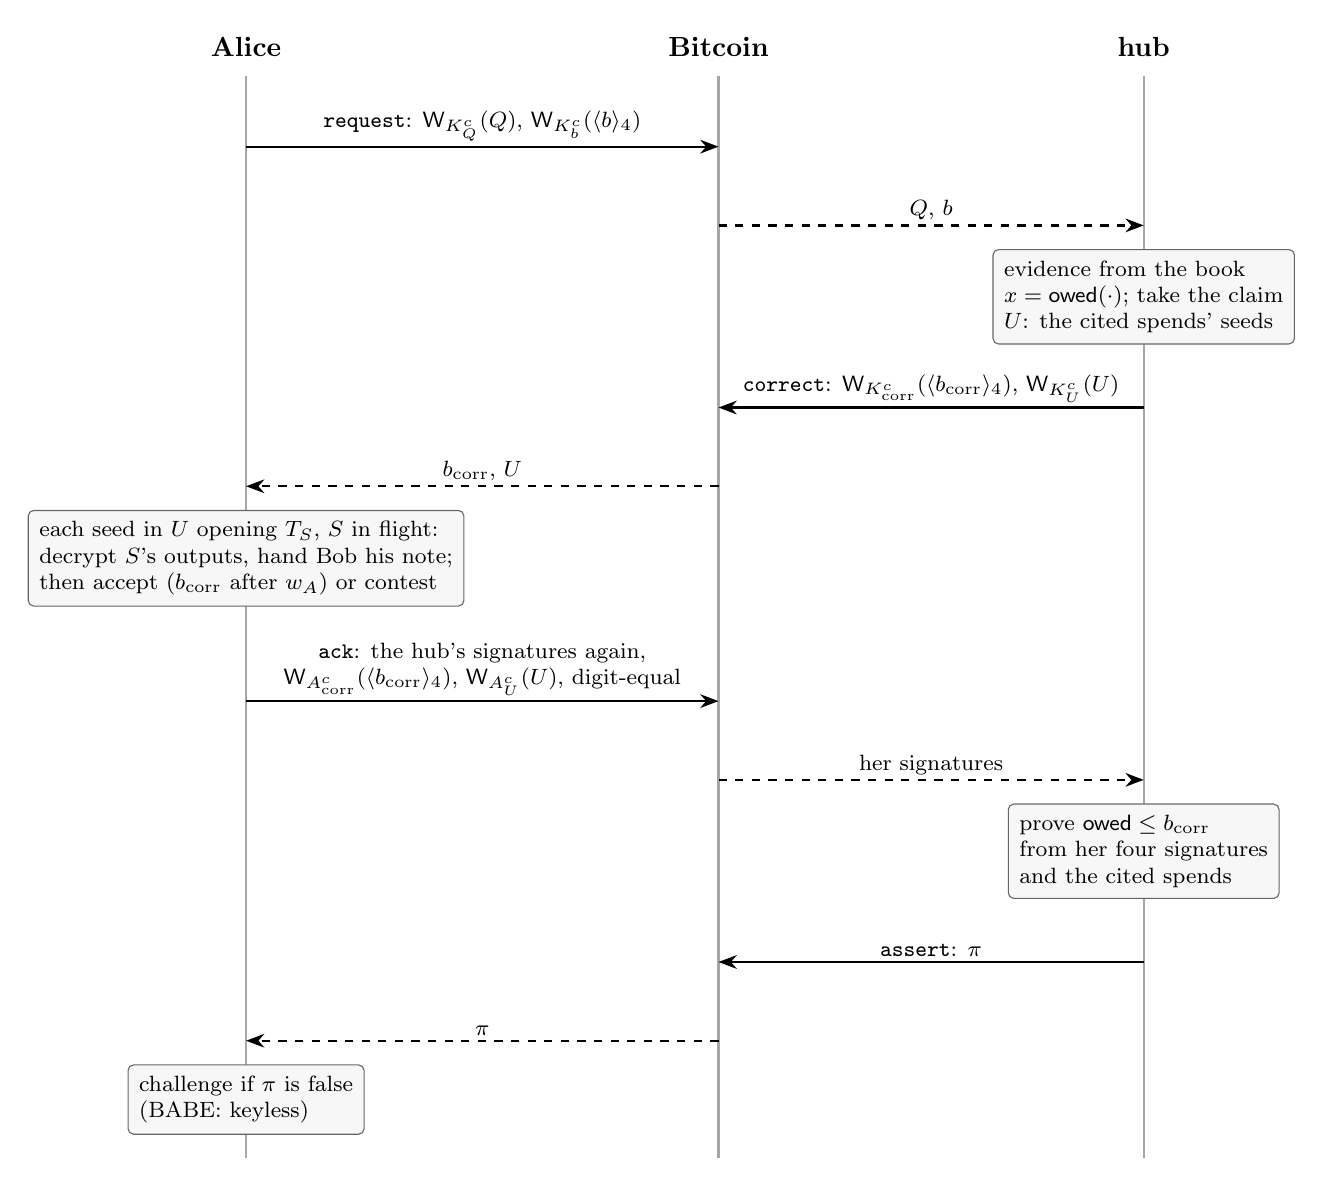
\begin{tikzpicture}[>=Stealth, font=\small,
  life/.style={draw=black!35, thick},
  box/.style={draw=black!60, fill=black!3, rounded corners=2pt, align=left, inner sep=4pt, font=\footnotesize},
  msg/.style={->, thick},
  lbl/.style={align=center, font=\footnotesize, inner sep=1.5pt}]
\coordinate (LA) at (2.6,0); \coordinate (LB) at (8.6,0); \coordinate (LH) at (14.0,0);
\node[font=\bfseries, anchor=base] at ($(LA)+(0,0.25)$) {Alice};
\node[font=\bfseries, anchor=base] at ($(LB)+(0,0.25)$) {Bitcoin};
\node[font=\bfseries, anchor=base] at ($(LH)+(0,0.25)$) {hub};
\coordinate (y) at (0,-0.9);
\draw[msg] (LA|-y) -- node[lbl, above] {\tx{request}: $\Wots_{\KQ}(Q)$, $\Wots_{\Kb}(\be{b}{4})$} (LB|-y);
\coordinate (y) at ($(y)+(0,-1.0)$);
\draw[msg, dashed] (LB|-y) -- node[lbl, above] {$Q$, $b$} (LH|-y);
\node[box, anchor=north] (h1) at ($(LH|-y)+(0,-0.3)$) {evidence from the book\\ $x = \owed(\cdot)$; take the claim\\ $U$: the cited spends' seeds};
\coordinate (y) at ($(h1.south)+(0,-0.8)$);
\draw[msg] (LH|-y) -- node[lbl, above] {\tx{correct}: $\Wots_{\Kcorr}(\be{\bcorr}{4})$, $\Wots_{\KU}(U)$} (LB|-y);
\coordinate (y) at ($(y)+(0,-1.0)$);
\draw[msg, dashed] (LB|-y) -- node[lbl, above] {$\bcorr$, $U$} (LA|-y);
\node[box, anchor=north] (a1) at ($(LA|-y)+(0,-0.3)$) {each seed in $U$ opening $T_S$, $S$ in flight:\\ decrypt $S$'s outputs, hand Bob his note;\\ then accept ($\bcorr$ after $w_A$) or contest};
\coordinate (y) at ($(a1.south)+(0,-1.2)$);
\draw[msg] (LA|-y) -- node[lbl, above] {\tx{ack}: the hub's signatures again,\\ $\Wots_{\Acorr}(\be{\bcorr}{4})$, $\Wots_{\AU}(U)$, digit-equal} (LB|-y);
\coordinate (y) at ($(y)+(0,-1.0)$);
\draw[msg, dashed] (LB|-y) -- node[lbl, above] {her signatures} (LH|-y);
\node[box, anchor=north] (h2) at ($(LH|-y)+(0,-0.3)$) {prove $\owed \le \bcorr$\\ from her four signatures\\ and the cited spends};
\coordinate (y) at ($(h2.south)+(0,-0.8)$);
\draw[msg] (LH|-y) -- node[lbl, above] {\tx{assert}: $\pi$} (LB|-y);
\coordinate (y) at ($(y)+(0,-1.0)$);
\draw[msg, dashed] (LB|-y) -- node[lbl, above] {$\pi$} (LA|-y);
\node[box, anchor=north] (a2) at ($(LA|-y)+(0,-0.3)$) {challenge if $\pi$ is false\\ (BABE: keyless)};
\coordinate (end) at ($(a2.south)+(0,-0.3)$);
\begin{scope}[on background layer]
\foreach \l in {LA,LB,LH} \draw[life] (\l) -- (\l|-end);
\end{scope}
\end{tikzpicture}
\caption{A contested exit. Dashed arrows: reading the chain. Silence
ends it: no \tx{correct}, $b$; no \tx{ack}, $\bcorr$; no \tx{assert},
$b$; a valid $\pi$ unchallenged, $\bcorr$; a false one challenged, $b$.}
\label{fig:exit}
\end{figure}

\textbf{A worked example.} Unit $u = 100$ sats. Alice's contract key $O$
holds $N_1$ of 70,000 and $N_2$ of 30,000 sats. She pays Bob 50,000 from
$N_1$:
\[
  S = \big(N_1;\ (O_B, 50{,}000),\ (O, 20{,}000)\big),
\]
signs it with its grant; the hub records $S$ but withholds $z_S$. Bob's
note never reaches him, and Alice still holds $N_1$, with $S$ in flight.
She exits with $b = 1000$ and $Q = (N_1, N_2;\ \text{fallback }
\pre{\sid_S}{8})$.
\begin{itemize}[nosep]
\item The hub is silent: \tx{request\_timeout} pays her 1000 units. Her
  payment to Bob never settled; no one else is owed anything.
\item The hub posts \tx{correct} with $\bcorr = 500$ and $U = (z_S, 0,
  \dots, 0)$. Alice reads $z_S$, decrypts Bob's note and hands it to
  him.
  Algorithm~1 kills $N_1$, revives $(\pre{\Ht{out}(\sid_S,
  \be{1}{4})}{16}, 20{,}000)$, and returns $\min(1000, \lfloor
  50{,}000/100\rfloor) = 500$. Whether she accepts or contests, she is
  paid 500 units and $r_A$.
\item The hub posts $\bcorr = 300$: she contests, it can't prove $\owed
  \le 300$, and she is paid 1000.
\item The hub posts $\bcorr = 500$ with a wrong word in $U$: she
  contests; $S$ doesn't count, $\owed = 1000$, and she is paid 1000.
\end{itemize}

\section{Costs}\label{sec:costs}

Estimates, scaled from version 0.1's measurements: about 12 vB per
witness item of one-time signatures with HASH160 chains, their scripts
included, and about 15 with SHA-256 (32-byte preimages and script
elements instead of 20, at the witness discount). None of this is
built.

\begin{center}
\begin{tabularx}{\linewidth}{lL}
\toprule
Item & Cost (est.) \\
\midrule
\tx{request} & $Q$ (137 bytes) and $b$ under her SHA-256 keys: 578 stack items, about 8.8 kvB \\
\tx{correct} & $\bcorr$ and $U$ (64 bytes) under the hub's HASH160 keys: $2(8 + 2) + 2(128 + 3) + 2 = 284$ items, about 3.5 kvB \\
\tx{ack} & the hub's signatures again (282 items, HASH160) and hers on the same values (282, SHA-256): 566 items, about 7.7 kvB \\
statement & no headers, no transaction parsing. Her four one-time signatures: about 430 SHA-256 chains, some 3,200 compressions, accelerated: about 1M cycles. Up to 4 BIP340 checks of $\alpha$ (accelerated). The BLS aggregate: two pairings and up to 4 hash-to-curve; the seeds: up to 4 scalar multiplications in $G_2$; RISC Zero has accelerated BLS12-381 forks, unmeasured here, perhaps 30--50M cycles, against 1.3M for all of v0.1's statement \\
payment & one round trip; the wallet checks $\tau$ and each encrypted signature, 2 pairings apiece, about a millisecond each with \tx{blst} \\
\bottomrule
\end{tabularx}
\end{center}

\textbf{Why seeds.} \tx{ack} carries two one-time signatures on every
byte, 8 stack items a byte. With 4 seeds (64 bytes) it uses 566 of
Bitcoin's 1,000 items; with 4 full scalars (128 bytes) it would need
1,078.

\textbf{Who pays.} The statement's cost is the hub's alone: only the
hub proves, and only when it corrects a claim and she contests. $w_H$
for \tx{assert} must cover its proving time. The user's costs are a
wallet's: BIP340 signatures, a few pairings per payment, and her moves
on chain, \tx{request} and perhaps \tx{ack}.

\section{Open questions}\label{sec:open}

\begin{itemize}[nosep]
\item \textbf{BLS in the guest.} Two pairings, up to four
  hash-to-curve and four $G_2$ multiplications on RISC Zero's
  accelerated BLS12-381 forks: to measure. It sets the hub's proving
  time and so $w_H$; it costs the user nothing.
\item \textbf{A keyless contest.} \tx{ack} needs Alice's keys within
  $w_A$ (\S\ref{sec:who}). Can a tower countersign without being able
  to sign other values off chain?
\item \textbf{Capacity.} $\mu + n + f \le 4$ bounds a claim, and so what
  an offline receiver has protected. Seeds leave room in \tx{ack} for
  more (7 fit); four keeps the transactions small.
\item \textbf{The hub and the guest must agree.} Every spend the hub
  records must be one the statement accepts. The hub should check at
  intake with the guest's own functions.
\item \textbf{Taking the claim and the evidence at once}, as one step
  of the book (\S\ref{sec:correct}, step 4).
\item \textbf{Fees.} Per payment (the issuer's revenue), and liquidity
  per unit time, as in the anchored L2.
\item \textbf{Restoring a wallet} needs each contract's nonce, from
  which its keys derive.
\item \textbf{The book} is one file rewritten on each change: fine for a
  testnet, not for volume.
\end{itemize}

\begin{thebibliography}{9}
\bibitem{lichen} waxwing, \emph{Lichen}, version 0.5, 2026.
\bibitem{ecash} m0wer, \emph{Lichen ecash: owner-bound ecash with local
  exits, enforced by Bitcoin}, version 0.2, November 2026.
\bibitem{delving} waxwing, \emph{Variable payout amounts for BABE, as
  applied to Lichen}, Delving Bitcoin, October 2026.
\bibitem{bls} D.~Boneh, B.~Lynn, H.~Shacham, \emph{Short signatures from
  the Weil pairing}, ASIACRYPT 2001; D.~Boneh, C.~Gentry, B.~Lynn,
  H.~Shacham, \emph{Aggregate and verifiably encrypted signatures from
  bilinear maps}, EUROCRYPT 2003.
\bibitem{erwig} A.~Erwig, S.~Faust, K.~Hostáková, M.~Maitra, S.~Riahi,
  \emph{Two-party adaptor signatures from identification schemes}, PKC
  2021 (the impossibility for unique signatures; to check).

\bibitem{bip340} P.~Wuille, J.~Nick, T.~Ruffing, \emph{BIP 340: Schnorr
  signatures for secp256k1}, 2020.
\end{thebibliography}

\end{document}
